\documentclass{article}
\usepackage[utf8]{inputenc}
\usepackage[margin=1in]{geometry}
\usepackage{graphicx}
\usepackage{float}
\usepackage{caption}
\usepackage{amsmath}
\usepackage{hyperref}
\usepackage{lipsum}
\usepackage{mwe}
\begin{document}
\title{PHY566 Group Project 2 Version B}
\author{Lingfei Zhao, Yuan Ji, Melissa Wu}
\maketitle

\begin{center}
\textit{\large Predator-Prey Model}\par
\end{center}
\bigskip
\noindent 1. \textbf{Quasi-Periodic Behaviour}\par
\smallskip
We aim to write a program that simulates a two-component predator-prey system (fish and shark) as discussed in class. Our world is two-dimensional with periodic boundary conditions. The parameters of our system are: the initial number of shark, initial number of fish, number of time steps for fish and shark to procreate, respectively, and the number of time steps for a shark to die of starvation.\par
We will briefly explain about the algorithm we used in making this program. In class, we were suggested to use five grids: "Fish", to store the presence or absence of a fish at a certain position, with -1 for no fish, and the age of the fish otherwise; "Shark", to store the same information for the shark; "Fishmove", to hold a record of whether the fish at a position has already been moved in the current timestep; "Sharkmove", to do the same for the sharks; and "Sharkstarve", which holds the amount of time since a shark's last meal. However, in our algorithm, we used two directories and one grid. The first directory stored the position and age of each fish, and the second directory store the position, age, and time since the last meal for each shark. The grid stores whether each position is empty, occupied with a fish, or occupied with a shark. What we do is operate through each fish in the fish directory first, changing their position in the grid when the fish moves. We then operate through the shark directory after that, again changing the grid accordingly. Since directories store more information than a single grid, we find that this is a faster way of running the program than having five grids.\par 
We track of the number of fish and shark at each time-step and plot the populations as a function of time. We also overlay the plot of the analytic equations from the Lotka-Vdterra equations, which model predator-prey behaviour. More about the analytic equations and their relation to our computational results will be explained later. Figure \ref{fig:graph} shows the fish and shark populations vs. time:\par
\begin{figure}[H]
\centering
\captionsetup{justification=centering, margin=3 cm}
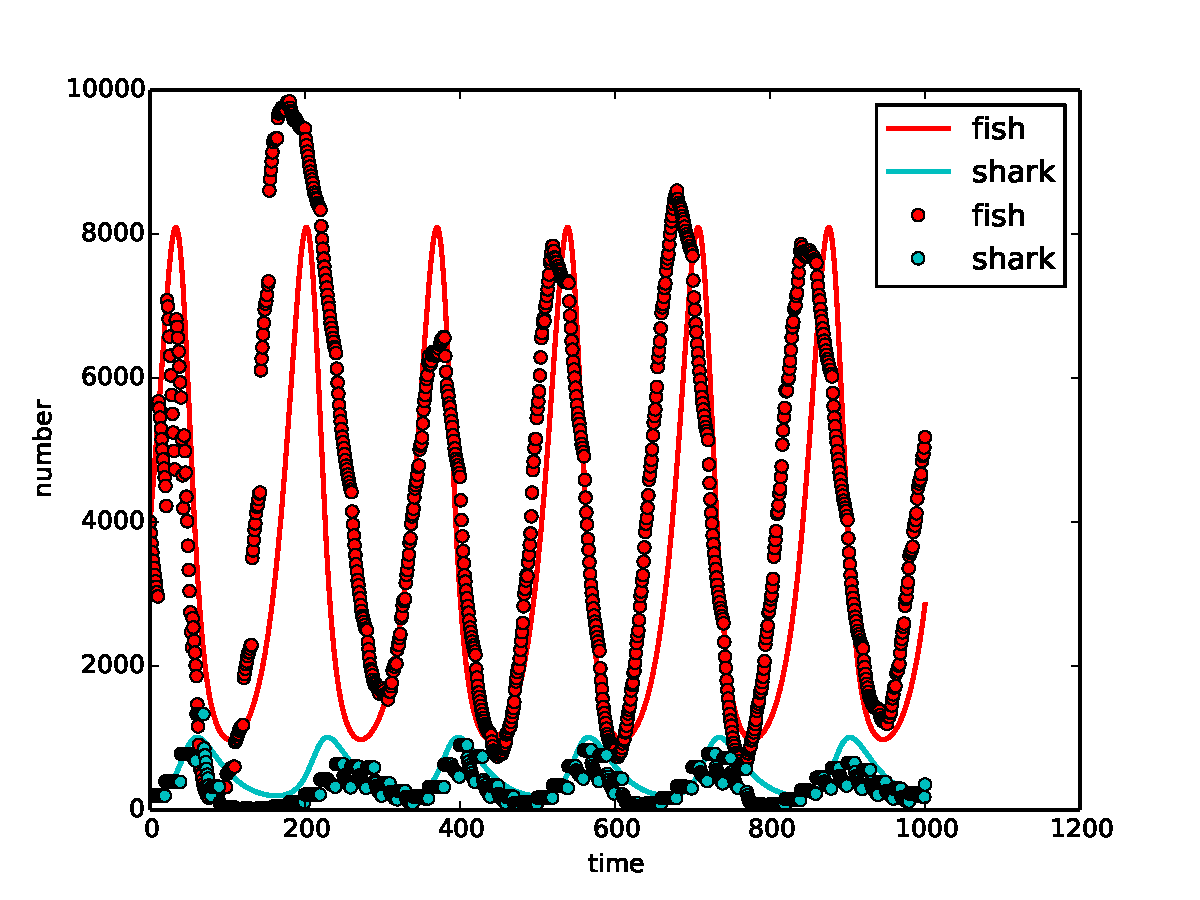
\includegraphics[width=10cm]{population.pdf}
\caption{Numbers of fish and shark versus time. We see a quasi-periodic behaviour of predator and prey.}
\label{fig:graph}
\end{figure}
The behaviour of the populations are not regular; we see that the amplitude of the fish population in the plot is switches between higher and lower values, with the maximum crest at approximately 8500 fish and minimum crest at approximately 5000 fish. The shark population, on the other hand, exhibits a more regular amplitude, reaching approximately (as a rough estimate from looking at the graph) 800 sharks each peak. This is interesting -- it seems that the sharks' maximum population is not noticeably dependent on the fish's maximum population. Both the shark and the fish population seem to regularly fail to reach the maximum predicted by the analytic equations, though their troughs align with the predicted troughs fairly regularly. The shark population reaches a peak at approximately the same relative time every period, which is just before the fish population reaches its lowest every period. We can see that right after the shark population hits its peak, the fish population hits its lowest, after which the shark population begins to decrease. Right after the fish population begins to rise, the shark population does as well -- so the shark population's graph is just a little bit phase-shifted fish population's. This makes sense, as the shark population needs some time to react to fluctuations in the fish population. This is the essence of the predator-prey model: if the prey population is high, the predator population thrives and increases as well, but once the number of predators increase, the number of prey decrease. This in turn causes the predators to die off, after which the prey begin to grow again -- all of which leads to the quasi-periodic model that is depicted in Figure \ref{fig:graph}.\par 
The initial parameters we used to reach this periodic behaviour in a 40 x 40 grid were: 300 initial fish, 20 initial sharks, 10 timesteps for the fish to breed, 20 timesteps for the shark to breed, and 10 timesteps for the shark to starve. So, the ratio between the initial numbers for the fish versus shark is 15:1, and the initial breeding ages for fish versus shark is 1:2. We can relate the observed computational results to analytic parameters in the Lotka-Vdterra equations. The differential equations are:\par
\begin{equation}
\frac{dx}{dt} = x(\alpha - \beta y)
\end{equation}
\begin{equation}
\frac{dy}{dt} = -y(\gamma - \delta x)
\end{equation}
Where $x$ is the number of prey, and $y$ is the number of predators. The descriptions of the parameters $\alpha$,$\beta$, $\gamma$, $\delta$ are as follows: $\alpha x$ is the growth term, which leads to exponential growth of the prey population in the absence of predators. $\beta yx$ is loss term, which depends on the number of predators and prey. $\gamma y$ is the loss term for predators, which leads to the exponential decay of predator population in the absence of prey. $\delta xy$ is the gain term for predators, which depends on both the predator and prey population. Now, we can find the parameters in the Lotka-Vdterra equations from the minimum and maximum predator and prey population values that we observe in Figure \ref{fig:graph} through the following method\footnote{Taken from \href{http://math.stackexchange.com/q/1853938}{this link}.}.\par
Every solution to the Lotka-Vdterra system is of the form\par
\begin{equation}
\delta x - \gamma \log x = \alpha \log y - \beta y + C
\label{eq:lv_solu}
\end{equation}
\noindent For a constant $C$. By setting the differential equations both to zero, we can see that $x$ is a minimum or maximum when $y = \frac{\alpha}{\beta}$, and $y$ is a minimum or maximum when $x = \frac{\gamma}{\delta}$. Let $x_{min}$ and $x_{max}$ be the minimum and maximum values that the prey reaches, respectively, and $y_{min}$ and $y_{max}$ be the minimum and maximum values that the predator reaches, respectively. Then we want to make $x_{min}$ and $x_{max}$ solve equation \ref{eq:lv_solu} for $y = \frac{\alpha}{\beta}$ and $y_{min}$ and $y_{max}$ solve equation \ref{eq:lv_solu} for $x = \frac{\gamma}{\delta}$. In other words, we want $x_{min}$ and $x_{max}$ to both solve
\begin{equation}
\delta x - \gamma \log x = \alpha \log (\alpha/\beta) - \alpha + C
\label{eq:xmin}
\end{equation}
and we want $y_{min}$ and $y_{max}$ to solve
\begin{equation}
\gamma + \gamma \log (\delta/\gamma) = \alpha \log y - \beta y + C
\label{eq:ymin}
\end{equation}
Thus, we see that $\delta x_{min} - \gamma \log x_{min} = \delta x_{max} - \gamma \log x_{max}$ and $\alpha \log y_{min} - \beta y_{min} = \alpha \log y_{max} - \beta y_{max}$. In other words, \begin{equation}
x_{min}\delta = \xi \gamma \hspace{0.5 cm} \textrm{and} \hspace{0.5 cm} y_{min} \beta = \eta \alpha
\end{equation}
where
\begin{equation}
\xi = h(x_{max}/x_{min}) \hspace{0.5 cm} \textrm{and} \hspace{0.5 cm} \eta = h(y_{max}/y_{min})
\end{equation}
respectively. We define $h(z)$ as
\begin{equation}
h(z) = \frac{\log z}{z - 1}
\end{equation}
Now, since $C$ needs to solve equation \ref{eq:xmin} when $x = x_{min}$ and equation \ref{eq:ymin} when $y = y_{min}$, they must yield the same value of $C$, in other words,
\begin{equation}
dx_{min} - c\log x_{min} + \alpha \log (\beta/\alpha) + \alpha = \gamma + \gamma \log (\delta/\gamma) + \beta y_{min} - \alpha \log y_{min}
\end{equation}
which can be written as
\begin{equation}
g(\eta) a = g(\xi) c
\end{equation}
where we define the function $g(z)$ as
\begin{equation}
g(z) = z - 1 - \log z
\end{equation}
So, solving these equations, we can write the Lotka-Vdterra parameters as:
\begin{equation}
\begin{split}
\alpha = g \circ h(x_{max}/x_{min}) \hspace{0.5 cm} \\
\beta = g \circ h(x_{max}/x_{min}) \cdot \frac{h(y_{max}/y_{min})}{y_{min}} \\
\gamma = g \circ h(y_{max}/y_{min}) \\
\delta = g \circ h(y_{max}/y_{min}) \cdot \frac{h(x_{max}/x_{min})}{x_{min}}
\end{split}
\end{equation}
Thus, the parameters we used in our Lotka-Vdterra equation to achieve the overlaying periodic curves were:\par
\bigskip
\noindent 2. \textbf{Snapshot configurations of our system}\par
Below is a link to a video of the shark-fish model, where the red squares are the fish and the blue squares are the sharks:\par
\href{https://github.com/LingfeiZhao/Group-Project-2b/blob/master/results/animationwithplot.mp4}{Video of shark-fish model}\par
And here are a few snapshots from the video:
\begin{figure}[htp]
    \centering
    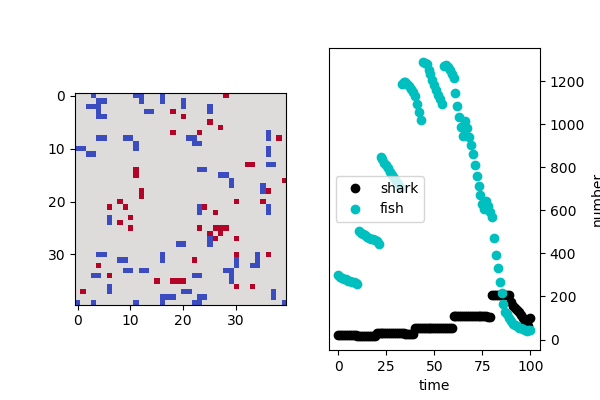
\includegraphics[width=0.4\textwidth]{99.png} 
    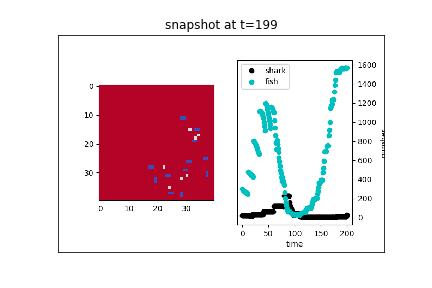
\includegraphics[width=0.4\textwidth]{199.png} 
    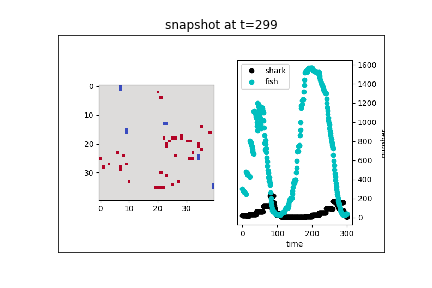
\includegraphics[width=0.4\textwidth]{299.png} 
    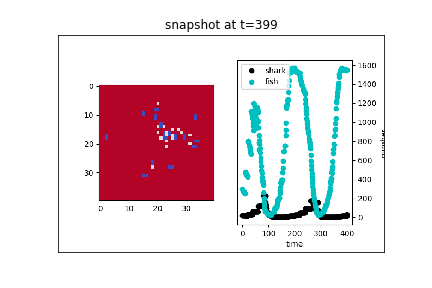
\includegraphics[width=0.4\textwidth]{399.png}
    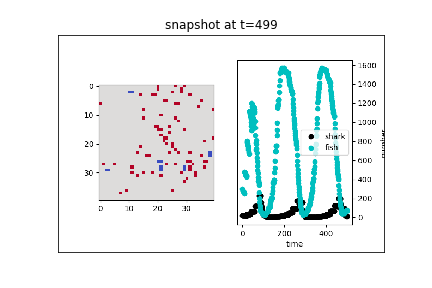
\includegraphics[width=0.4\textwidth]{499.png}
    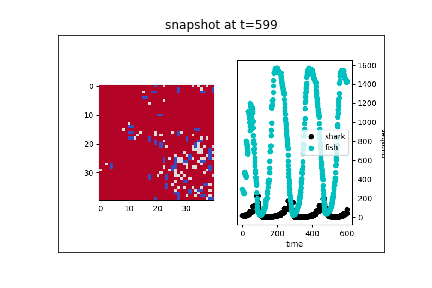
\includegraphics[width=0.4\textwidth]{599.png}
    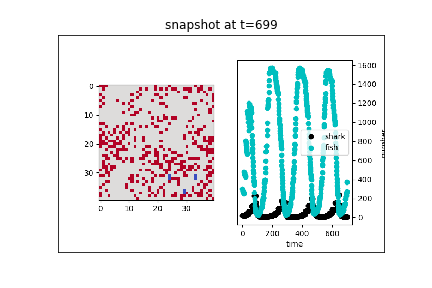
\includegraphics[width=0.4\textwidth]{699.png}
    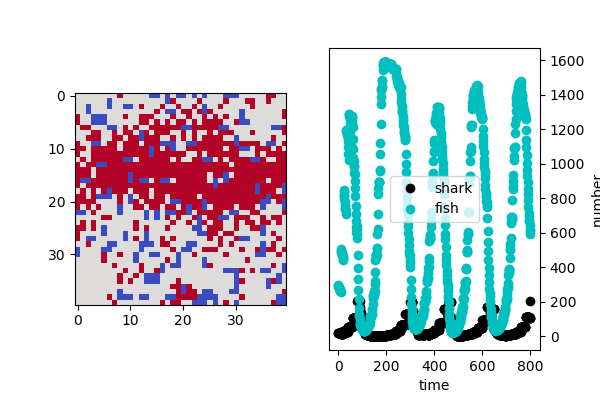
\includegraphics[width=0.4\textwidth]{799.png}
    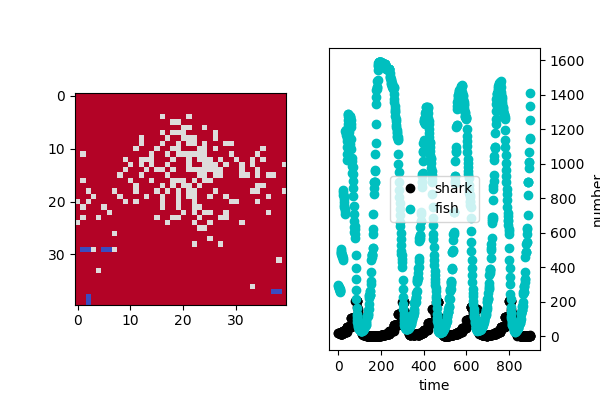
\includegraphics[width=0.4\textwidth]{899.png}
    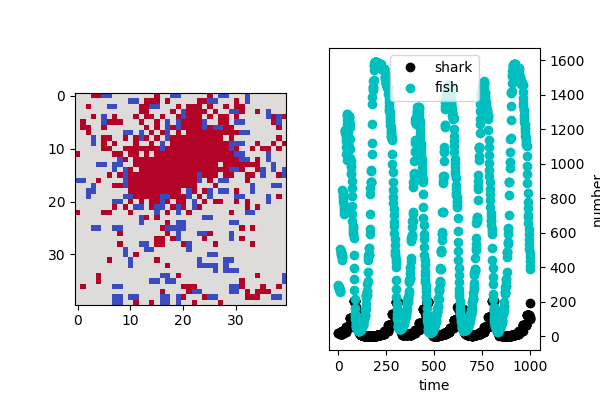
\includegraphics[width=0.4\textwidth]{999.png}
    \caption*{Figure 2}
\end{figure}


Looking at the video, we can see that the number of fish increase significantly before the number of sharks begin to noticeably increase -- the grid gets filled up with red squares before the increasing presence of blue squares eats away at the red ones. This is evident from the adjacent plot as well. It is also interesting to note that the video depicts how quickly sharks that have little to no surrounding fish die off, as we are able to observe entire regions of blue dots disappear in almost a single timestep. Another phenomenon that can be seen is that in some periods, the fish almost completely flood the grid before the shark population is able to catch up and eat the fish. While the maximum number of fish varies, as one can tell in the video, Figure \ref{fig:graph} tells us that the maximum number of sharks stays approximately the same. In some periods, the shark population is almost dangerously low; the at 0:06 and other snapshots, there are less than 5 sharks left in a grid of
40 x 40. However, we still observe multiple times that the shark population manages to rise despite that.\par
\bigskip
\noindent Github repository: \url{https://github.com/LingfeiZhao/Group-Project-2b}
\end{document}
